\section{Incomputabilidade}

\begin{frame}[fragile]{Existência de funções incomputáveis}

    \begin{itemize}
        \item É possível demonstrar que o conjunto de todas as funções de inteiros positivos em
            inteiros positivos não é enumerável

        \item Por outro lado, o conjunto de todas as máquinas de Turing é enumerável: cada 
            máquina pode ser especificada por uma sequência de quádruplas, que equivale a 
            uma cadeira finita de símbolos de um alfabeto finito, e o conjunto de tais cadeias
            é enumerável

        \item Deste modo, existem funções que não são Turing computáveis

        \item Especificar exemplos de tais funções, contudo, não é tarefa trivial
    \end{itemize}

\end{frame}

\begin{frame}[fragile]{Enumeração das máquinas de Turing}

    Para ilustrar o processo de enumeração das máquinas de Turing, considere a máquina abaixo,
    que atribui o valor $1$ para qualquer $k$-upla:

    \vspace{0.3in}

    \begin{figure}[h]
        \centering
        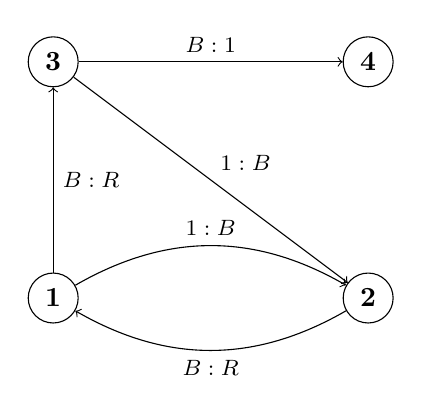
\begin{tikzpicture}
            \node[draw,circle] (q1) at (0, 0) { $\mathbf{1}$ };
            \node[draw,circle] (q2) at (4, 0) { $\mathbf{2}$ };
            \node[draw,circle] (q3) at (0, 3) { $\mathbf{3}$ };
            \node[draw,circle] (q4) at (4, 3) { $\mathbf{4}$ };

            \draw[->] (q1) edge[bend left] node[anchor=south] { \footnotesize $1 : B$ } (q2);
            \draw[->] (q1) edge node[anchor=west] { \footnotesize $B : R$ } (q3);
            \draw[->] (q2) edge[bend left] node[anchor=north] { \footnotesize $B : R$ } (q1);
            \draw[->] (q3) edge node[anchor=south west] { \footnotesize $1 : B$ } (q2);
            \draw[->] (q3) edge node[anchor=south] { \footnotesize $B : 1$ } (q4);

        \end{tikzpicture}
    \end{figure}

\end{frame}

\begin{frame}[fragile]{Enumeração das máquinas de Turing}

    \begin{itemize}
        \item A máquina apresentada pode ser representada pela seguinte lista de quádruplas
        \[
            q_1S_0Rq_3, \ \ q_1S_1S_0q_2, \ \ q_2S_0Rq_1, \ \ q_3S_0S_1q_4, \ \ q_3S_1S_0q_2
        \]

        \item Tal especificação, embora correta, não permite a enumeração de todas as máquinas
            de Turing

        \item Para tal fim, da mesma forma que foi feito para as máquina de Turing, é preciso
            especificar precisamente a representação de uma máquina por meio de uma lista
            de quádruplas
    \end{itemize}

\end{frame}

\begin{frame}[fragile]{Especificação para a lista de quádruplas}

    \begin{enumerate}[(a)]
        \item O estado de menor número ($\mathbf{1}$) é o \textbf{estado inicial}

        \item O estado de maior número ($\mathbf{n + 1}$) será o \textbf{estado de parada}: para 
            este estado, não há instruções nem quádruplas

        \item Para cada estado, exceto para o estado de parada, existe uma quádrupla iniciando
            com $q_iS_j$, com $i = 1, 2, \ldots, n, j = 0, 1$

        \item De acordo com \textbf{(c)}, se as quádruplas forem listadas em ordem crescente de
            $i$ e de $j$, os dois primeiros símbolos de cada quádrupla são previsíveis, e poderão
            ser omitidos

        \item Os estados $q_i$ devem ser representados pelo inteiro $i$, os símbolos $S_j$ por
            $j + 1$ (para evitar o zero) e as instruções $L$ e $R$ pelos inteiros $3$ e $4$,
            respectivamente
    \end{enumerate}

    \textbf{Observação}: uma máquina de Turing descrita por uma lista de quádruplas que atende a
        especificação acima corresponde a um inteiro positivo, de acordo com a codificação baseada
        no Teorema Fundamental da Aritmética.
\end{frame}

\begin{frame}[fragile]{Exemplo de codificação de uma máquina de Turing}

    \begin{itemize}
        \item A lista de quádruplas da máquina que retorna um para qualquer $k$-upla dada abaixo
        \[
            q_1S_0Rq_3, \ \ q_1S_1S_0q_2, \ \ q_2S_0Rq_1, \ \ q_3S_0S_1q_4, \ \ q_3S_1S_0q_2
        \]
        não atende à especificação

        \item Observe que as duas primeiras especificações são atendidas: ($\mathbf{1}$) é o 
            estado final e ($\mathbf{n + 1} = \mathbf{4}$) é o estado final

        \item Contudo, não existe uma quádrupla iniciando com $q_2S_1$, violando \textbf{(c)}:
            para corrigir isto, basta adicionar uma nova quádrupla, que mantém o símbolo e 
            vai para o estado final:
        \[
            q_1S_0Rq_3, \ \ q_1S_1S_0q_2, \ \ q_2S_0Rq_1,\ \ q_2S_1S_1q_4,\ \ q_3S_0S_1q_4, \ \ q_3S_1S_0q_2
        \]
        
    \end{itemize}

\end{frame}

\begin{frame}[fragile]{Exemplo de codificação de uma máquina de Turing}

    \begin{itemize}
        \item Aplicando o critério \textbf{(d)}, a lista se reduz à
        \[
            Rq_3, \ \ S_0q_2, \ \ Rq_1,\ \ S_1q_4,\ \ S_1q_4, \ \ S_0q_2
        \]

        \item Usando o critério \textbf{(e)} obtêm-se:
        \[
            4, 3, 1, 2, 4, 1, 2, 4, 2, 4, 1, 2
        \]

        \item Codificando esta máquina o resultado é o inteiro positivo:
        \[
            2^4\cdot 3^3\cdot 5\cdot 7^2\cdot 11^4\cdot 13\cdot 17^2\cdot 19^4\cdot 23^2\cdot 29^4\cdot 31\cdot 37^2
        \]

        \item Em notação decimal, a máquina seria representada pelo inteiro
        \[
            12047279224912544432864883318480
        \]
    \end{itemize}

\end{frame}

\begin{frame}[fragile]{Enumerabilidade das máquinas de Turing}

    \begin{itemize}
        \item A codificação acima permite enumerar as máquinas de Turing $M_1, M_2, M_3, \ldots$

        \item Observe que nem todo inteiro positivo corresponde à uma máquina de Turing: isto
            depende de sua decomposição em fatores primos

        \item Além disso, nem toda sequência $a_k$ formada pelos números de $1$ 
            a $4$ corresponde a uma máquina de Turing

        \item Para que tal sequência represente uma máquina de Turing, ela precisa atender três
            critérios:
            \begin{enumerate}[i.]
                \item $|a_k| = 4n$, para algum inteiro positivo $n$
                \item $a_i\in [1,4]$, se $i$ é ímpar (uma das quatro instruções possíveis)
                \item $a_j\in [1,n + 1]$, se $j$ é par (um dos $n+1$ estados possíveis)
            \end{enumerate}
            
        \item Assim, a codificação apresentada é uma função parcial dos inteiros positivos que
            enumera as máquinas de Turing
    \end{itemize}

\end{frame}

\begin{frame}[fragile]{Exemplos de máquinas de Turing}

    \begin{itemize}
        \item Considere a máquina 
        \[
            (1, 1, 1, 1) = 2\cdot 3\cdot 5\cdot 7 = 210
        \]

        \item O fluxograma correspondente seria

    \begin{figure}[h]
        \centering
        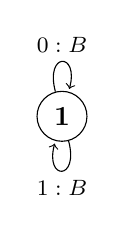
\begin{tikzpicture}
            \node[draw,circle] (q1) at (0, 0) { $\mathbf{1}$ };

            \draw[->] (q1) edge[loop above] node { \footnotesize $0 : B$ } (q1);
            \draw[->] (q1) edge[loop below] node { \footnotesize $1 : B$ } (q1);

        \end{tikzpicture}
    \end{figure}


        \item A partir da configuração inicial, esta máquina apaga o traço que está no bloco e
            retorna para o estado ($\mathbf{1}$)

        \item A partir daí ela não faz mais nada, jamais atingindo a configuração final 
            ($\mathbf{2}$)
    \end{itemize}

\end{frame}

\begin{frame}[fragile]{Exemplos de máquinas de Turing}

    \begin{itemize}
        \item Considere a máquina 
        \[
            (2, 1, 1, 1) = 2^2\cdot 3\cdot 5\cdot 7 = 420
        \]

        \item O fluxograma correspondente seria

    \begin{figure}[h]
        \centering
        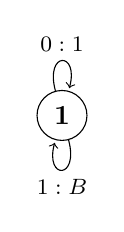
\begin{tikzpicture}
            \node[draw,circle] (q1) at (0, 0) { $\mathbf{1}$ };

            \draw[->] (q1) edge[loop above] node { \footnotesize $0 : 1$ } (q1);
            \draw[->] (q1) edge[loop below] node { \footnotesize $1 : B$ } (q1);

        \end{tikzpicture}
    \end{figure}

        \item A partir da configuração inicial, esta máquina apaga o traço que está no bloco e
            retorna para o estado ($\mathbf{1}$)

        \item Em seguida, ele reescreve o traço e permanece em ($\mathbf{1}$), reiniciando o ciclo,
            sem jamais parar
    \end{itemize}

\end{frame}

\begin{frame}[fragile]{Exemplos de máquinas de Turing}

    \begin{itemize}
        \item Seja a máquina 
        \[
            (1, 2, 1, 1) = 2\cdot 3^2\cdot 5\cdot 7 = 630
        \]

        \item O fluxograma correspondente seria

    \begin{figure}[h]
        \centering
        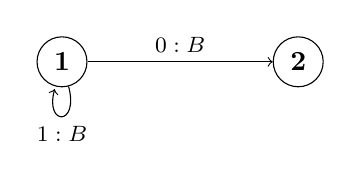
\begin{tikzpicture}
            \node[draw,circle] (q1) at (0, 0) { $\mathbf{1}$ };
            \node[draw,circle] (q2) at (3, 0) { $\mathbf{2}$ };

            \draw[->] (q1) edge node[anchor=south] { \footnotesize $0 : B$ } (q2);
            \draw[->] (q1) edge[loop below] node { \footnotesize $1 : B$ } (q1);

        \end{tikzpicture}
    \end{figure}

        \item A partir da configuração inicial, esta máquina apaga o traço que está no bloco e,
            ao o reexaminar, segue para o estado ($\mathbf{2}$)

        \item Como ($\mathbf{2}$) é o estado final, e o quadrado está em branco, a máquina parou
            em um configuração final que não é a padrão

        \item As três máquinas exemplificadas correspondem aos menores inteiros positivos 
            associados à uma máquina de Turing (isto é, $M_1, M_2, M_3$), e todas elas computam
            a função vazia 
    \end{itemize}

\end{frame}

\begin{frame}[fragile]{Função diagonal}

    \begin{block}{Definição}
        Seja $f_i$ a função computada pela $i$-ésima máquina de Turing. A \textbf{função diagonal}
        $d$ é definida por
        \[
            d(n) = \left\lbrace \begin{array}{ll}
                2,& \mbox{se}\ f_n(n)\ \mbox{é definida e}\ f_n(n) = 1, \\
                1,& \mbox{caso contrário}
            \end{array}\right.
        \]
    \end{block}

\end{frame}

\begin{frame}[fragile]{Incomputabilidade da função diagonal}

    \begin{block}{Teorema}
        A função diagonal não é Turing computável.
    \end{block}

    \begin{block}{Demonstração}
        Suponha, por contradição, que a função diagonal seja Turing computável. Assim, para algum
        $m$ positivo, $d(n) = f_m(n)$, para qualquer $n$ positivo. 

        \vspace{0.1in}

        No caso em que $n = m$, porém, surge uma contradição: se $f_m(n) = 1$ então, por definição,
        $d(m) = 2$; caso contrário, se $f_m(n)\neq 1$ ou se $f_m(n)$ não for definida, $d(m) = 1$.
        Em todos os casos, $d(m) \neq f_m(m)$, o que contradiz a hipótese de $d$ ser Turing
        computável.
     
        \vspace{0.1in}

        Portanto, a função diagonal $d$ não é Turing computável.
    \end{block}

\end{frame}

\begin{frame}[fragile]{Problema da parada}

    \begin{itemize}
        \item Se a Tese de Turing estiver correta, a função diagonal não seria efetivamente 
            computável

        \item Porém, a princípio, parece ser possível computar a função $d$ para qualquer
            argumento $n$

        \item Por exemplo, para as três primeiras máquinas de Turing, apresentadas anteriormente,
            $f_1, f_2$ e $f_3$ são iguais a função vazia, de modo que $d(1) = d(2) = d(3) = 1$

        \item Se $f_n(m)$ está definida para $m$, o valor de $d(m)$ será $1$, se $f_n(m) = 1$, ou
            $d(m) = 2$, se $f_(m) \neq 1$

        \item Se $f_n(m)$ parar em uma configuração final diferente da padrão, $d_n(m) = 1$

        \item A situação difícil de identificar e computar acontece quando $f_n(m)$ não para

        \item Não existe, até o presente momento, um procedimento mecânico uniforme que permita,
            para qualquer Máquina $M_i$, decidir se a função $f_i$ para ou não para o argumento
        $m$

        \item Este é o problema da parada
    \end{itemize}

\end{frame}

\begin{frame}[fragile]{Função de parada}

    \begin{block}{Definição}
        A \textbf{função de parada} de dois argumentos $h(m, n)$ é definida por
        \[
            h(m, n) = \left\lbrace \begin{array}{ll}
                1,& \mbox{se}\ f_m(n)\ \mbox{para em alguma configuração}, \\
                2,& \mbox{caso contrário}
            \end{array}\right.
        \]
    \end{block}

    \vspace{0.2in}

    \begin{block}{Teorema}
        A função de parada não é Turing computável.
    \end{block}

\end{frame}
